\chapter*{Anhang}
\label{sec:Anhang}

\section*{Aufgabenstellung}

\section*{Interviews}

\section*{Assessment}

\section*{Projektplan, Protokolle}

\section*{Übersichtausschnitt der Auftragsaufteilung}

\newpage
\section*{Aufgabe a: Berechnung AP Transistorschaltung}
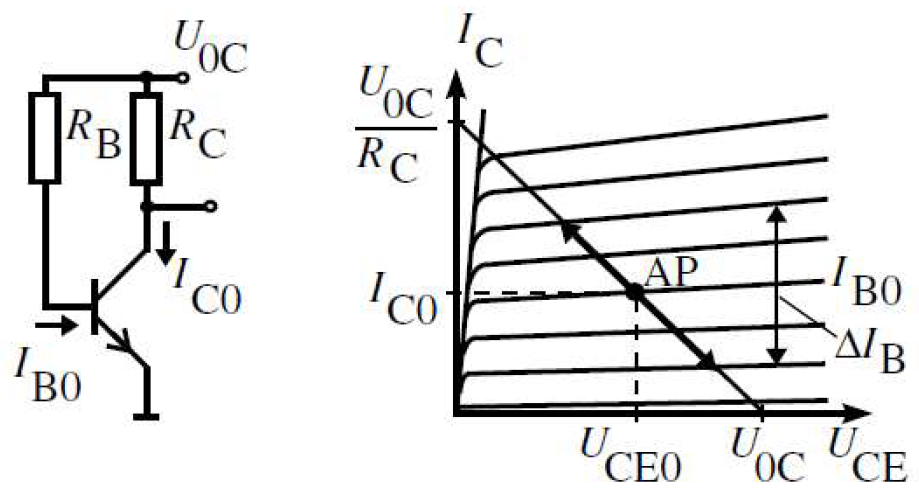
\includegraphics[width=1\textwidth]{images/emitterStufe.png}

Die Speisung VDD(U0C) sei 5V

\begin{enumerate}
\item Wie gross wird der Kollektorstrom IC0 im Arbeitspunkt, wenn die Arbeitspunkt-Spannung
UCE0=VDD/2 betragen soll?
\item Wie gross wird der Basisstrom IB0 für den Arbeitspunkt, wenn Sie einen npn-Transistor zur Verfügung haben und dieser genau den mittleren Stromverstärkungsfaktor hFE aufweist?
\item Wie gross wird die zu erwartende Basis-Emitter-Spannung VBE0 bei Ihrem Arbeitspunkt?
\end{enumerate}

\newpage
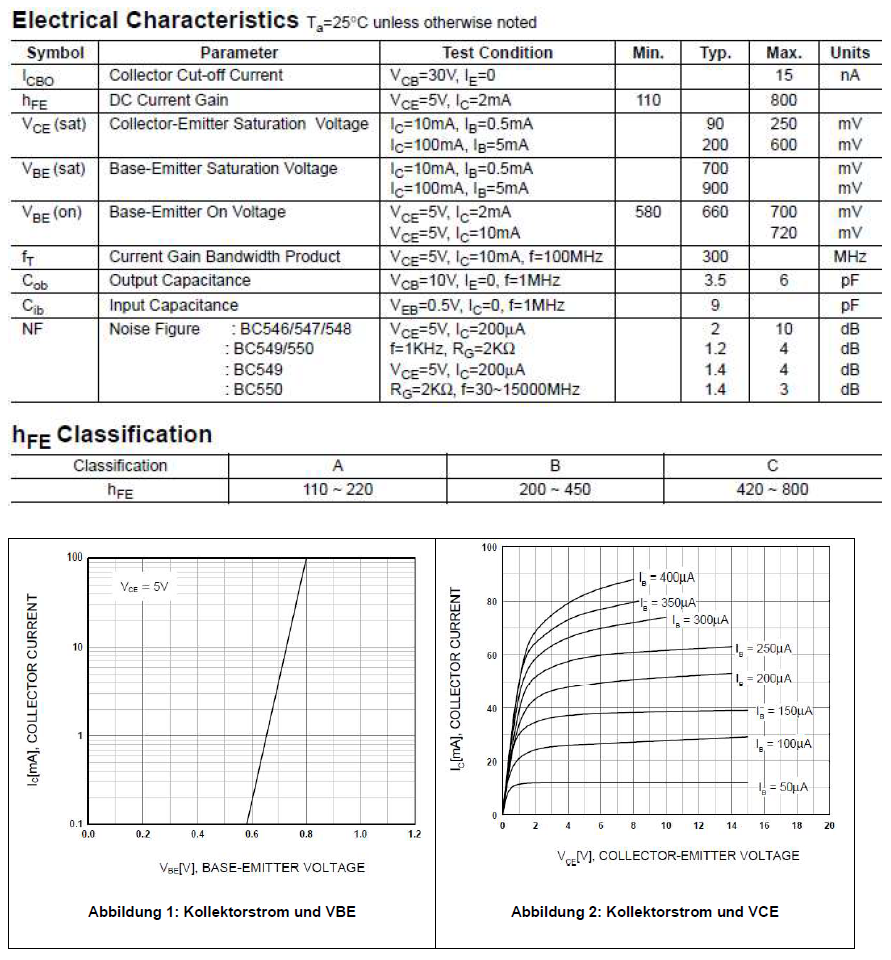
\includegraphics[width=1\textwidth]{images/datasheetBC547.png}
\newpage
\section*{Aufgabe b: Berechnung Operationsverstärkerschaltung T0454}
Gegeben ist folgende Schaltung (T0454) eines Operationsverstärkers mit geschalteten Widerständen

\includegraphics[width=1.2\textwidth]{images/opAmp.png}

Der Opamp sei ideal, d.h. er habe unendliche Verstärkung und Eingangswiderstand,keine Offsetspannung. 
Die Schalter S2, S1 und S1 sind ideal, d.h. es fliesst kein Strom, wenn sie offen sind und es fällt keine Spannung ab, wenn sie geschlossen sind.

Schalterstellung: S2, S1 und S0 geschlossen; Vin1 = 0V, Vin2 = 1V

Für unsere Anwendung soll Vout -1.75 Volt und If 1.75 mA betragen, wobei R2 = 1kOhm, R1 = 2kOhm und R0 4kOhm beträgt.

Wie gross muss Rf sein?
\newpage
\section*{Aufgabe c: Beantwortung E-Mail}
From: pirmin.meier@company.ch\\
To: peter.hasler@company.ch\\

Hallo lieber Peter,\\\\
hiermit sende ich, wie angekündigt, die von Dir so dringend benötigten Informationen. 
Bezüglich der Weiterentwicklung im Bereich der Abteilung Forschung und Entwicklung kann ich Dir folgendes mitteilen. Ich habe mit dem Bereichsleiter T\&E unserer Division gestern ein intensives Gespräch darüber geführt. Mit Sicherheit konnte er mir auch noch nicht viel bestätigen, was aber schon feststeht und sich sicher nicht mehr ändern wird, ist folgendes: Die jetzigen Forschung und Entwicklung Räumlichkeiten werden aufgegeben und ein neues, grösseres Labor am bestehenden Firmengebäude angebaut. Dieser Anbau dürfen wir aber frühestens 2022 erwarten. Die jetzigen zur Verfügung stehenden Messmittel werden zum grossen Teil ersetzt werden, wir werden neue Digital Signal Analyzer und Kathodenstrahloszilloskope mit sechs Kanälen erhalten. Die jetzigen werden, beginnend Ende 2017 etappenweise ersetzt. Genauere Informationen dazu später. Bezüglich dem personellen Ausbau von unserem Team ist momentan eine Personalsteigerung zwischen 15-25\% in Diskussion. Diese Personen werden, beginnend 2018 rekrutiert und in die Abteilung eingegliedert.
Um noch Deine Frage wegen des zu verwendenden Transistors für die Emitterstufe (Schaltung T0455) zu beantworten, ich denke ein off-the-shelf BC547 wird dazu locker reichen. \\
Was ich nun von Dir noch benötige sind folgende Informationen:
Wie gross ist der Feedback-Widerstand des Op-Amp der Schaltung T0454?
Wann genau wirst Du im Herbst deinen WK leisten, damit ich die Personalplanung anpassen kann?
Wie ist der genaue Arbeitsstand im Gerdo-Projekt?
Wie viel Zeit hast Du in etwa aufgewendet, um den Messbericht von Pavel zu korrigieren? Ich brauche diese Angabe für die zukünftige Planung.\\\\
Vielen Dank für Deine Antwort\\\\
Gruss Pirmin

Pirmin Meier\\
El. Ing. HTL\\
Abteilungsleiter F \& E\\
The Company AG\\
6300 Zug\\
Switzerland
   
\textbf{Messbericht Schaltungsteil T0453} Verstärkerschaltung 20.04.17

Der Schaltung vom Schaltungsteil T0453 wurde von mir (Pavel Datsyuk) am 20.04.17 mit Umgebungsbedingungen normal (22 Grade Celsius, 60 Prozentes relativer Luftfeuchtigkeiten) augemessen. Der Resultat der Messung ware wie erwartet positiv ausgefallen. Ich haben die Messunge exakt gleich gemacht auch noch einmal bei 
\section*{Aufgabe e: Ausfüllen Kreuzworträtsel}
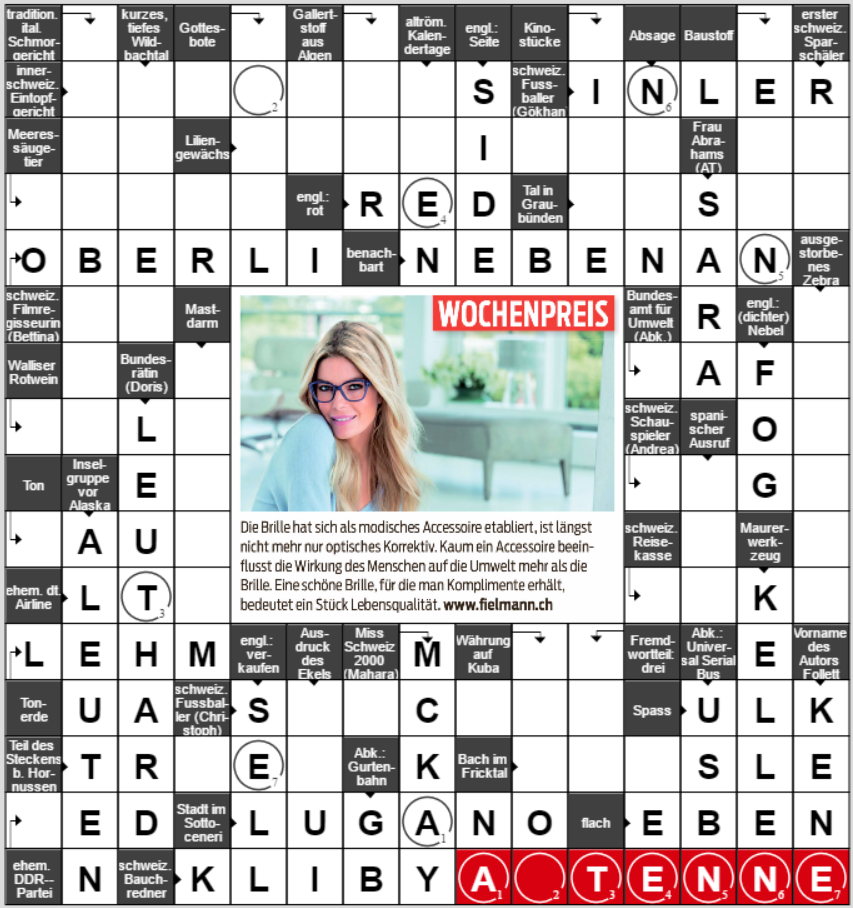
\includegraphics[width=1.2\textwidth]{images/Kreuzwortraetsel.png}
\newpage

\section*{Projektplan, Protokolle}

Datum:03.04.2017\\
Ort: HSR Rapperswil

Teilnehmer: Steve Gerome Kamga, Pascal Horat, Gökhan Kaya\\
Sitzungsleiter: Pascal Horat

Thema: Projektauftrag definieren und verstehen
\begin{enumerate}

\item Ablauf und Aufgabeplanung, Eröffnung der Sitzung 

\item  Verteilung der Aufgaben während der Sitzung
\begin{itemize}
\item Gerome: Sitzungsprotokole
\item Gökhan: Schreiben
\item Pascal: Schreiben 
\end{itemize}

\item Kontext des Projekts definieren un mögliche Fragen zum Projektsbeginn erklären.

\item Mögliche Probleme und Schwierigkeiten erwahnen

\item Regeldokument erstelen : es geht darum, allgemeiner Regeln festzulegen, welche für die Teamarbeit als verbinlich gelten.

\item Projektziele festlegen und Teamrolle gemäss Teamreview 2 beschreiben.

\item Mögliche voraussetzung für einen erfolreichen Projektmanagement definieren

\item Benötigte Literatur: HSR Projektauftrag.docx   

\item Zusammenfassung

\end{enumerate}

Nächste Sitzung: 13.04.2017




\newpage

\section*{Projektplan, Protokolle}

Datum:13.04.2017\\
Ort: HSR Rapperswil

Teilnehmer: Steve Gerome Kamga, Pascal Horat, Gökhan Kaya\\
Sitzungsleiter: keiner

Thema: Klärung der Aufgabenstellung

\begin{enumerate}

\item Ablauf und Aufgabeplanung, Eröffnung der Sitzung 

\item  Verteilung der Aufgaben während der Sitzung
\begin{itemize}
\item Gerome: Sitzungsprotokole
\item Gökhan: Interviewleitfaden erstellen
\item Pascal: MS-Projekt
\end{itemize}

\item GrobePlanung mit Microsoft Projekt erstellen: Damit jeder von uns immer immer auf das Projekt zugreifen kann.

\item Detailplanung erstellen

\item Baseline erstellen und als .pdf speichern

\item Interviewleitfaden erstellen: vorhandener Fragekatalog mit Fragekatalog von Dozent erweitern, Raster für Koordinaten des Befragten erstellen, Frage hinzufügen ob Befragter genannt werden will.

\item Latex-Vorlage Projektbericht organisieren

\item Benötigte Literatur: 

\item Zusammenfassung

\end{enumerate}

Nächste Sitzung: 19.04.2017

\newpage
\section*{Projektplan, Protokolle}

Datum:19.04.2017\\
Ort: HSR Rapperswil

Teilnehmer: Steve Gerome Kamga, Pascal Horat, Gökhan Kaya\\
Sitzungsleiter: keiner

Thema: Plannung un Vorgehen des Interviews (1)

\begin{enumerate}

\item Ablauf und Aufgabeplanung, Eröffnung der Sitzung 

\item  Verteilung der Aufgaben während der Sitzung
\begin{itemize}
\item Gerome: Sitzungsprotokole
\item Gökhan: 
\item Pascal: 
\end{itemize}

\item	Projektbericht Template erstellen

\item  interviewleitfaden herstellen:  Mit Hilfe internets zehn Schlüsselkompetenzen auswählen.

\item 	interviewPartner für Beschaffung der Kernkompetenzen notieren: Jeder notiert sich 3 mögliche Partner, die er kontaktieren könnte. damit wir   sicherstellen können, dass jeder am Schluss Kontakt mit ca. 2 Partnern hatte.

\item 	Terminvorschlag mit mögliche Interviewpartner festlegen:  Die Termine sind in unserem Auftragsdokument in Excel unter Tab «Projektpartner» zu notieren.

\item	Antwortformulare Einfordern : Formulare mit Namen der befragten Person beschriften und unter OneDrive/TKI /ProjektAC/Befragung abspeichern.


\item Latex-Vorlage Projektbericht organisieren

\item Benötigte Literatur: Simon 2002   \cite{simon2002entwicklung}

\item Zusammenfassung

\end{enumerate}

Nächste Sitzung: 05.05.2017

\newpage
\section*{Projektplan, Protokolle}

Datum:05.05.2017\\
Ort: HSR Rapperswil

Teilnehmer: Steve Gerome Kamga, Pascal Horat, Gökhan Kaya\\
Sitzungsleiter: keiner

Thema: Auswertung der Interview

\begin{enumerate}

\item Ablauf und Aufgabeplanung, Eröffnung der Sitzung 

\item  Verteilung der Aufgaben während der Sitzung
\begin{itemize}
\item Gerome: Sitzungsprotokole
\item Gökhan: 
\item Pascal: 
\end{itemize}

\item	Projekt anpassen gemäss plan.


\item 	Übersichtsdokument der Kompetenzen erstellen :In diesem Dokument sollten alle Antworten der Formulare eingetragen und dann ausgewertet werden. Dieses Dokument wird optimalerweise direkt in Projektbericht verfasst.

\item 	Kernkompetenzen ermitteln.

\item 	An Projektbericht weiter schreiben

\item Benötigte Literatur: Simon 2002   \cite{simon2002entwicklung}

\item Zusammenfassung

\end{enumerate}

Nächste Sitzung: 14.05.2017

\newpage
\section*{Projektplan, Protokolle}

Datum:14.05.2017\\
Ort: HSR Rapperswil

Teilnehmer: Steve Gerome Kamga, Pascal Horat, Gökhan Kaya\\
Sitzungsleiter: keiner

Thema: überlegung über Beobachtungsinstrument
\begin{enumerate}

\item Ablauf und Aufgabeplanung, Eröffnung der Sitzung 

\item  Verteilung der Aufgaben während der Sitzung
\begin{itemize}
\item Gerome: Sitzungsprotokole
\item Gökhan: 
\item Pascal: 
\end{itemize}


\item  Die wichtigsten Kernkompetenzen selektieren:
\begin{itemize}
\item Analytisches und systematisches Denken
\item Lernbereitschaft und Lernfähigkeit
\item Selbstmanagement und Selbstorganisation 
\end{itemize}

\item mögliche Ideen zum Beobachtungsinstrument vorschlagen: es geht darum zwei übungen zu entwickeln,  mit denen sich die fünf von uns gewählten Kernkompetenzen herauskristalisiernen lassen

\item Erzeugung Von Übungen zum Testen der Kernkompetenzen

\item Powerpoint Vorlage für die Präsentation vorbereiten	

\item Probanten für den Test der Kernkompetenzen auswählen


\item Benötigte Literatur: 

\item Zusammenfassung

\end{enumerate}

Nächste Sitzung: 19.05.2017

\newpage
\section*{Projektplan, Protokolle}

Datum:19.05.2017\\

Ort: HSR Rapperswil

Teilnehmer: Steve Gerome Kamga, Gökhan Kaya\\

Sitzungsleiter: keiner

Thema: Erstellung der Projektpräsentation
\begin{enumerate}

\item Ablauf und Aufgabeplanung, Eröffnung der Sitzung 

\item  Verteilung der Aufgaben während der Sitzung
\begin{itemize}
\item Gerome: 
\item Gökhan: 
\end{itemize}

\item PowerPoint erzeugen und einrichten

\item Präsentation üben


\item Benötigte Literatur: 

\item Zusammenfassung

\end{enumerate}

Nächste Sitzung: 01.06.2017



\newpage
\section*{Projektplan, Protokolle}

Datum:01.06.2017\\
Ort: HSR Rapperswil

Teilnehmer: Steve Gerome Kamga, Pascal Horat, Gökhan Kaya\\
Sitzungsleiter: keiner

Thema: Bewertung der Probanten
\begin{enumerate}

\item Ablauf und Aufgabeplanung, Eröffnung der Sitzung 

\item  Verteilung der Aufgaben während der Sitzung
\begin{itemize}
\item Gerome: Sitzungsprotokole
\item Gökhan: 
\item Pascal: 
\end{itemize}



\item Resultate der einzelnen Probanten analysieren, interpretieren und schön darstellen 		

\item 	Projektauftrag weiter schreiben

\item 	Bewertung der Ergebnissen von Beobachtungsinstrument


\item Benötigte Literatur

\item Zusammenfassung

\end{enumerate}

Nächste Sitzung: 07.06.2017

\newpage
\section*{Projektplan, Protokolle}

Datum:07.06.2017\\
Ort: HSR Rapperswil

Teilnehmer: Steve Gerome Kamga, Pascal Horat, Gökhan Kaya\\
Sitzungsleiter: keiner

Thema: Projektbericht fertigstellen
\begin{enumerate}

\item Ablauf und Aufgabeplanung, Eröffnung der Sitzung 

\item  Verteilung der Aufgaben während der Sitzung
\begin{itemize}
\item Gerome: Sitzungsprotokole
\item Gökhan: Auswertung der ÜBUNGEN Schreiben
\item Pascal: Bericht erweitern
\end{itemize}

\item Bewertungsergebnisse zur Lernbereitschaft und Lernfähigkeit

\item Verfassung der Übungsauswertung, Kapitel 3 (Klärung Projektauftrag)  sowie Zusammenfassung im Projektbericht 

\item Auswertung Assesment in Projektbericht

\item Interview ausbauen und Reflexion Verfassen

\item Schlussfolgerungen, Ausblicke und Empfehlungen verfassen 

\item Zusammenfassung

\end{enumerate}

Nächste Sitzung: 8.06.2017

\newpage

\section*{Übersichtausschnitt der Auftragsaufteilung}

%\begin{tabular}{ | l | l | l |}
 %\begin{tabular}{ | p{7cm} | p{4cm} | p{2cm} |}
 \begin{longtable}{ | p{7cm} | p{4cm} | p{2cm} |}
   \hline
   \textbf{Auftrag} & \textbf{Verfasser} & \textbf{Zeit[min]}   \\
   \hline  		
    Microsoft Project einrichten & Gerome & 60 \\ \hline
    Detailplanung erstellen & Pascal & 180 \\ \hline
    Baseline erstellen  & Pascal & 30 \\ \hline
    Interviewleitfaden erstellen& Gökhan,Gerome & 180 \\ \hline
    LaTeX-Vorlage Projektbericht organisieren & Pascal, Gökhan & 100 \\ \hline
    Lernbilanz 2 & Pascal, Gerome,Gökhan & \\ \hline
    lernbilanz 3 & Pasacl, Gerome,Gökhan &  \\ \hline
    Projektbericht Template erstellen & Gökhan & 120 \\ \hline
    Partner für Beschaff. Kernkomp. notieren & Pascal,Gerome,Gökhan & 30 \\ \hline
    Projektplan anpassen gemäss Angaben & Pascal & 120 \\ \hline
    Termine Interviewpartner festlegen & Pascal, Gerome, Gökhan & 30 \\ \hline
    Formulare versenden & Pascal, Gerome Göhkan & 15 \\ \hline
    Antwortformulare Einfordern & Pascal, Gerome, Gökhan & 10 \\ \hline
    Übersichtsdok. Kompetenzen erstellen & Gökhan & 60 \\ \hline    
    Kernkompetenzen ermitteln & Gerome,Gökhan & 10 \\ \hline   
    an Projektbericht schreiben & Gökhan & 90 \\ \hline   
    Punkt c im File AuftragAC\_ersteLektion.png erledigen &  &  \\ \hline    
    Aufgabe entwickeln oder finden um die Kernkompetenz Lernbereitschaft zu testen  & Pascal &  \\ \hline   
    Aufgabe entwickeln oder finden um die Kernkompetenz Selbstmanagement zu testen  & Gökhan & 90 \\ \hline  
    Teamsitzungsprotokolle erstellen & Gerome & 100 \\ \hline    
    Analyse Projektauftrag in main.tex einbringen, Vorlage in HSR\_Projektauftrag.docx & Gerome, Gökhan & 20\\ \hline   
    Übersicht erstellen wer wie viel Zeit für was investiert hat im Projekt TKI & Gerome & 60\\ \hline   
    Commit-History in 06vorgehen.tex schön formatieren & Gerome & 30 \\ \hline 
    Auswertung der Übung in Projektbericht verfassen  & Pascal, Gökhan & 480 \\ \hline   
Auswertung des Assessments in Projektbericht verfassen & Pascal, Gökhan & 200 \\ \hline  
Zusammenfassung auf Seite 2 in Projektbericht verfassen     & Pascal &  \\ \hline   
Commit-History aus Git extrahieren und in Latex erweitern, in Anhang von Projektbericht verschieben     & Gerome & 30 \\ \hline
 Verzeichnisse (Kapitel 1) einfügen in Projektbericht    &  &  \\ \hline  
 Einleitung erweitern    & Pascal &  \\ \hline   
 Kapitel 3 verfassen (Klärung Projektauftrag)    & Pascal &  \\ \hline
 Formattierung Projektbericht verbessern (inkl. Unterschriften in Kapitel 4)    & Pascal, Gökhan &  \\ \hline  
 Kapitel 7 Interview ausbauen  & Pascal, Gökhan &  \\ \hline   
 Kapitel 11 Reflexion verfassen & Pascal, Gökhan &  \\ \hline    
 Kapitel 12 Schlussfolgerungen, Ausblicke und Empfehlungen    verfassen & Pascal, Gökhan &  \\ \hline  
 Erklärung Urheberschaft einfügen & Pascal & 30 \\ \hline   
 Anhang in Projektbericht erweitern & Gerome &  \\ \hline     
 Tabelle Übersichtausschnitt der Auftragsaufteilung in Projektbericht aktualisieren anhand \_Aufträge.xlsx    & Gerome &  \\ \hline    
     &  &  \\ \hline  
   
%\end{tabular}
\end{longtable}